\documentclass[12pt,letterpaper]{amsart}
\usepackage[letterpaper,margin=1in]{geometry}
\usepackage[T1]{fontenc}
\usepackage{mathptmx}
\usepackage{amsmath,amssymb,amsthm,mathtools}
\usepackage{booktabs,array,enumitem,tabularx,tikz}
\usetikzlibrary{arrows.meta,positioning}
\usepackage[hidelinks]{hyperref}
\allowdisplaybreaks[2]
\setcounter{section}{8}
\numberwithin{equation}{section}
\newtheorem{theorem}{Theorem}[section]
\newtheorem{proposition}[theorem]{Proposition}
\newtheorem{lemma}[theorem]{Lemma}
\newtheorem{corollary}[theorem]{Corollary}
\theoremstyle{definition}
\newtheorem{definition}[theorem]{Definition}
\newtheorem{example}[theorem]{Example}
\theoremstyle{remark}
\newtheorem{remark}[theorem]{Remark}
\newcommand{\St}{\mathrm{St}}
\newcommand{\triv}{\mathbf 1}
\newcommand{\tr}{\operatorname{tr}}
\newcommand{\Ind}{\operatorname{Ind}}
\newcommand{\EP}{\operatorname{EP}}
\newcommand{\PW}{\operatorname{PW}}
\newcommand{\ST}{\mathcal{ST}}
\newcommand{\Ann}{\operatorname{Ann}}
\newcommand{\Hom}{\operatorname{Hom}}
\newcommand{\Ext}{\operatorname{Ext}}
\newcommand{\vol}{\operatorname{vol}}
\newcommand{\ev}{\operatorname{ev}}
\newcommand{\status}[1]{\textup{[\textsc{#1}]}}
\title[Supertempered distributions on $\mathrm{SL}_2(F)$]{Supertempered distributions on $\mathrm{SL}_2(F)$:\\ a research report toward Section 9 of Draft 3}
\author{Prepared for David Joyner by Claude (Fable, Anthropic)}
\date{November 24, 2026. Proposal for review. Nothing in the repository has been changed.}
\begin{document}
\maketitle

\section*{What this report is}
This is a proposal for the mathematics of Section 9 of \emph{A hitch-hiker's guide to invariant distributions on $\mathrm{SL}_2$ over a $p$-adic field}, Draft 3. I read the main file, the four modules, the 1994 Section 9 (and Section 4.2 of the 1994 notes, which it uses), the revision log and the style guide. Section 9 below is written so that statements can be lifted into the paper. Its numbering is the proposed numbering. Sections 10 to 12 are about the paper, not for the paper: errors found in earlier sections, the status of every input, and a recommended organization.

\subsection*{Status tags}
Every statement carries one of these tags.
\begin{itemize}[leftmargin=*]
\item \status{Proved}: derived here from the stated inputs. I checked the derivation, and where a formula has numbers in it I checked them by an exact computation (a short script, available on request).
\item \status{Cited}: a published result. \status{Cited, consulted} means I read the statement in the source during this pass. \status{Cited, memory} means I did not, and the reference must be audited.
\item \status{Conditional}: depends on the Schwartz trace identification that Sections 5 to 7 of Draft 3 leave open.
\item \status{Heuristic}: an estimate or expectation, not a proof.
\end{itemize}
No novelty is claimed anywhere. Most of the structure below is the rank-one case of theorems of Harish-Chandra, Casselman, Kazhdan, Bernstein--Deligne--Kazhdan, Arthur, Herb and Schneider--Stuhler. For three items I found no source in a limited search: the general split descent criterion (Corollary \ref{cor:descent}), the comparison of the two splittings (Theorem \ref{thm:twosplit}), and the counterexamples of Subsection \ref{sub:counter}. That is a statement about my search, not about the literature.

\subsection*{The main findings in one page}
\begin{enumerate}[leftmargin=*]
\item \textbf{Herb's theorem has a complete elementary proof in rank one.} A tempered virtual character is supertempered exactly when it lies in the span of the discrete series characters and the three differences $D_\eta=\Theta_{\pi_\eta^+}-\Theta_{\pi_\eta^-}$. The proof uses only the classification, the Jacquet modules and Casselman's character theorem (Theorem \ref{thm:herb}).
\item \textbf{Four functions on the torus must be kept apart.} They are the normalized split restriction $h_\Theta$ of Section 8, the Jacquet character $J_\Theta$, the weak constant term $\Theta^w$, and the compact defect $h_\Theta-J_\Theta$. They agree for induced characters and differ for every discrete series (Table \ref{tab:four}).
\item \textbf{Three classes are strictly nested}: elliptic support $\subsetneq$ cuspidal (zero Jacquet character) $\subsetneq$ supertempered (zero weak constant term). Steinberg separates the last two. A depth-zero supercuspidal character separates the first two, because it equals $|t-t^{-1}|^{-1}-1$ on split elements near $I$ (Proposition \ref{prop:sc}).
\item \textbf{The exceptional coordinates of Sections 3 and 5 to 7 describe one quotient with two splittings.} The quotient is the elliptic space $R(G)/R_{\rm ind}(G)$. The tempered coordinate $b=\tr\St$ of Sections 5 to 7 picks out the supertempered characters. The algebraic coordinate $d_{\St}=\tr\St-\tr\triv$ of Section 3 picks out the Bernstein--Deligne--Kazhdan elliptic part. They differ by $\tfrac12[I(|\cdot|)]$ on the Steinberg line and nowhere else (Theorem \ref{thm:twosplit}).
\item \textbf{The weak constant term of a distribution is the induced part of Section 8.} Every invariant distribution in a block is uniquely $\tfrac12\,D^w_B\circ(\cdot)^{(B)}+\Theta^{\rm st}$ with $\Theta^{\rm st}$ supertempered, and $D^w_B$ is the locally constant function of Theorem 8.6 of Draft 3 (Theorem \ref{thm:decomp}).
\item \textbf{The singular behavior at $\pm I$ is governed by one number.} Near $t=1$, $h_\Theta(a(t))=\tfrac12 w(\Theta)+c_0(\Theta)\,|t-t^{-1}|$. Here $c_0$ is the coefficient of the trivial nilpotent orbit and $w$ counts Whittaker models. The split restriction is locally constant at $I$ exactly when $c_0(\Theta)=0$. This extends Theorem 8.8 of Draft 3 beyond one block, and it shows that the Steinberg obstruction can be cancelled by supercuspidals (Corollary \ref{cor:descent}).
\item \textbf{Explicit elliptic values from the tree.} For the unramified quadratic character, $\Theta_{\pi_\pm}(\gamma)=\pm(V_0(\gamma)-V_1(\gamma))$ on elliptic $\gamma$, where $V_i$ counts fixed vertices of type $i$ (Theorem \ref{thm:tree}). The Euler--Poincar\'e form on a quadratic block is computed from the infinite dihedral Hecke algebra (Proposition \ref{prop:EP}).
\item \textbf{Hecke-finite is blockwise center-finite}, and it does not imply ``virtual character.'' Parameter derivatives of characters are Hecke-finite. So one lemma of the 1994 Section 9 is false as stated, but its corollary survives (Proposition \ref{prop:hecke}).
\item \textbf{Outside virtual characters, neither decay nor elliptic support implies supertemperedness.} There is a tempered admissible invariant distribution with finite Bernstein support, zero density on the whole regular split set, and nonzero weak constant term (Example \ref{ex:poisson}).
\end{enumerate}

\section{Supertempered distributions (proposed Section 9)}
Throughout, $F$ is a finite extension of $\mathbb Q_p$ with $p$ odd. Characteristic zero is needed for Herb's theorem and for the local character expansion. Notation is that of Draft 3: $G=\mathrm{SL}_2(F)$, $K=K_0=\mathrm{SL}_2(\mathcal O)$, $a(t)=\operatorname{diag}(t,t^{-1})$, $B=AN$, normalized induction $I(\chi)$, $c=q+q^{-1}$, $u=z+z^{-1}$. Write $A^0=a(\mathcal O^\times)$ and $v$ for the valuation. Let $K_1=gK_0g^{-1}$ with $g=\operatorname{diag}(\varpi,1)$, the other maximal compact subgroup, and $\mathcal I=K_0\cap K_1$ the Iwahori subgroup. Haar measure on $G$ gives $K_0$ volume one.

\subsection{Six notions}\label{sub:six}
The words below are often used as if they were synonyms. In rank one each can be made completely explicit.

\begin{definition}\label{def:six}
Let $R(G)$ be the complexified Grothendieck group, $R_{\rm temp}(G)$ the span of the irreducible tempered classes, and $R_{\rm ind}(G)$ the span of the classes $[I(\chi)]$ for all quasicharacters $\chi$.
\begin{enumerate}[label=(\alph*),leftmargin=*]
\item A \emph{tempered invariant distribution} is a conjugation-invariant continuous functional on $\mathcal C(G)$. A \emph{tempered virtual character} is an element of $R_{\rm temp}(G)$, viewed as a distribution.
\item A tempered virtual character $\Theta$ is \emph{supertempered} if for every $r>0$ the function\[|\Delta_G(\gamma)|^{1/2}\,|\Theta(\gamma)|\,(1+\sigma(\gamma))^r\]is bounded on the regular set of every Cartan subgroup \cite{He94}. In $G$ only the split torus is noncompact, so the condition is that $h_\Theta(a(t))(1+|v(t)|)^r$ is bounded, where $h_\Theta(a)=|\Delta_G(a)|^{1/2}\Theta(a)$.
\item An irreducible tempered representation is \emph{elliptic} if its character is not identically zero on the regular elliptic set \cite{Ar93}.
\item The \emph{elliptic virtual characters} of Arthur are the $\Theta(M,\sigma,r)=\tr\bigl(R(r,\sigma)I_P(\sigma)\bigr)$ with $\sigma$ in the discrete series of $M$ and $r$ a regular element of the $R$-group. For $G$ they are the discrete series characters ($M=G$) and the three $D_\eta$ ($M=A$, $\sigma=\eta$, $r=w$).
\item A virtual character is \emph{cuspidal} if its normalized Jacquet module vanishes in $R(A)$, that is $r_B\Theta=0$. A \emph{supercuspidal character} is the character of an irreducible supercuspidal representation.
\item A distribution has \emph{elliptic support} if it is represented by a locally integrable function that vanishes on the regular split set. The \emph{elliptic class} of $\Theta\in R(G)$ is its image in $\overline R(G)=R(G)/R_{\rm ind}(G)$.
\end{enumerate}
\end{definition}
\begin{example}
Both $\pi_\eta^+$ and $\pi_\eta^-$ are elliptic tempered representations in the sense of (c), by Theorem \ref{thm:tree} below. Neither character is supertempered, since each has weak constant term $\eta$. Only their difference is. So ``elliptic representation'' and ``elliptic virtual character'' must not be merged. The Steinberg character is supertempered and is not cuspidal. The trivial character is not tempered, yet $\Theta_{\St}-\Theta_{\triv}$ is twice the natural algebraic representative of the elliptic class of $\St$ (Theorem \ref{thm:twosplit}).
\end{example}

\subsection{Constant terms: four functions on the torus}\label{sub:four}
Section 8 of Draft 3 separates the ordinary restriction, the normalized split restriction and the Jacquet-module constructions, and leaves their comparison open. In rank one the comparison is a table.

For a finite-length representation $\pi$ let $r_B(\pi)=\pi_N\otimes\delta_B^{-1/2}$ be the normalized Jacquet module, a finite-dimensional representation of $A\simeq F^\times$. Its \emph{exponents} are the characters that occur. For tempered $\pi$ let $r_B^w(\pi)$ be the sum of the generalized eigenspaces with unitary exponents. Herb's weak constant term is the character of the maximal tempered quotient of the normalized Jacquet module \cite[Section 2]{He94}, which has the same character. Put
\[
J_\pi=\tr r_B(\pi),\qquad \Theta_\pi^w=\tr r_B^w(\pi),\qquad h_\pi(a)=|\Delta_G(a)|^{1/2}\Theta_\pi(a)\quad(a\in A_{\rm reg}),
\]
and extend by linearity. The test-function side is Harish-Chandra's map $f\mapsto f^{(B)}$, with $f^{(B)}(a)=\delta_B(a)^{1/2}\int_N\int_K f(kank^{-1})\,dk\,dn$. It equals $F_f^A$ on $A_{\rm reg}$, lies in $C_c^\infty(A)$, and satisfies
\begin{equation}\label{eq:adj}
\Theta_{I(\chi)}(f)=\int_A\chi(a)f^{(B)}(a)\,da=\tfrac12\int_A(\chi+\chi^{-1})(a)\,f^{(B)}(a)\,da .
\end{equation}

\begin{proposition}[Casselman's theorem in rank one]\label{prop:cass}
\status{Cited, memory; checked on four families} Let $\Theta\in R(G)$. Then\[h_\Theta(a(t))=J_\Theta(a(t))\ \text{ for }|t|<1,\qquad h_\Theta(a(t))=J_\Theta(a(t^{-1}))\ \text{ for }|t|>1 .\]
\end{proposition}
This is \cite{Ca77}. Every regular $a(t)$ with $|t|\ne1$ is strictly contracting for $B$ or for the opposite Borel subgroup, so the theorem covers all of $A$ outside $A^0$. I checked it against the explicit characters of $I(\chi)$, $\St$, $\triv$ and $\pi_\eta^\pm$. On $A^0$ the two functions can differ. Call $E_\Theta=h_\Theta-J_\Theta$ on $A^0_{\rm reg}$ the \emph{compact defect}. It is well defined because $J_\Theta|_{A^0}$ is Weyl-invariant in every case below.

\begin{table}[htbp]\centering\small
\caption{The four functions on $A$. Here $|t|<1$ in the third column and $|t|=1$ in the last two. The supercuspidal row is for $\pi=\operatorname{c-Ind}_{K_0}^G\sigma$ with $\sigma$ cuspidal of dimension $q-1$ (Proposition \ref{prop:sc}).}\label{tab:four}
\begin{tabular}{@{}lllll@{}}\toprule
$\Theta$ & $J_\Theta$ & $h_\Theta$, $|t|<1$ & weak constant term & $E_\Theta$ on $A^0_{\rm reg}$\\\midrule
$I(\chi)$, $\chi$ unitary & $\chi+\chi^{-1}$ & $\chi+\chi^{-1}$ & $\chi+\chi^{-1}$ & $0$\\
$\pi_\eta^\pm$ & $\eta$ & $\eta$ & $\eta$ & $0$\\
$D_\eta$ & $0$ & $0$ & $0$ & $0$\\
$\St$ & $|t|$ & $|t|$ & $0$ & $1-|t-t^{-1}|$\\
$\triv$ & $|t|^{-1}$ & $|t|^{-1}$ & not defined & $|t-t^{-1}|-1$\\
supercuspidal $\pi$ & $0$ & $0$ & $0$ & $\omega_\pi(\pm1)(1-|t-t^{-1}|)$ on $\pm(1+\mathfrak p)$\\\bottomrule
\end{tabular}
\end{table}
The Jacquet characters come from the geometric lemma $r_B\,i_B\chi=\chi+\chi^{-1}$ in $R(A)$. At a quadratic point each constituent embeds in $I(\eta)$, so by Frobenius reciprocity each has a nonzero Jacquet module, and each gets one copy of $\eta$. At $|\cdot|^{\pm1}$ the trivial representation has $r_B(\triv)=\delta_B^{-1/2}=|\cdot|^{-1}$, which leaves $|\cdot|$ for Steinberg. The Steinberg row is the reason for the word ``weak'': its ordinary constant term is $|t|\neq0$ and its weak constant term is zero.

\begin{proposition}[Bohr-mean formula]\label{prop:bohr}\status{Proved}
Let $\Theta$ be a tempered virtual character. Then $h_\Theta(a(t))-\Theta^w(a(t))=\beta\,q^{-|v(t)|}$ for $v(t)\ne0$, where $\beta$ is the coefficient of $\Theta_{\St}$ in $\Theta$. Consequently, for every unitary character $\chi$ of $F^\times$, the coefficient of $\chi$ in $\Theta^w$ is
\[
\lim_{N\to\infty}\frac1N\sum_{m=1}^N\int_{\mathcal O^\times}h_\Theta\bigl(a(\varpi^mx)\bigr)\,\overline{\chi(\varpi^mx)}\,dx .
\]
\end{proposition}
\begin{proof}
By Proposition \ref{prop:cass}, $h_\Theta=J_\Theta$ for $|t|<1$. By Table \ref{tab:four} the only non-unitary exponent of a tempered irreducible representation is the exponent $|\cdot|$ of Steinberg. The Weyl symmetry of $h_\Theta$ gives $|t|>1$. The limit formula is orthogonality of characters on $\mathcal O^\times$ followed by a Ces\`aro mean in $m$, and the term $\beta q^{-m}$ has mean zero.
\end{proof}
So the weak constant term is the almost periodic part at infinity of the normalized split restriction. It is not the restriction itself, and it says nothing about $A^0$.

\subsection{Herb's theorem in rank one}\label{sub:herb}
Herb proved, for every connected reductive $p$-adic group in characteristic zero, that a tempered virtual character is supertempered if and only if all its weak constant terms along proper parabolic subgroups vanish \cite[Theorem 2.5]{He94}, that the supertempered virtual characters are spanned by Arthur's elliptic virtual characters \cite[Theorem 3.1]{He94}, and that a supertempered virtual character vanishing on the elliptic set is zero \cite[Theorem 3.2]{He94}. \status{Cited, consulted} For $G=\mathrm{SL}_2(F)$ all three statements can be proved directly.

\begin{theorem}[Rank-one Herb theorem]\label{thm:herb}\status{Proved, given the classification, Proposition \ref{prop:cass} and local boundedness of $h_\Theta$}
For a tempered virtual character $\Theta=\sum_\pi a_\pi\Theta_\pi$ of $G$ the following are equivalent.
\begin{enumerate}[label=(\roman*),leftmargin=*]
\item $\Theta^w=0$.
\item $\Theta$ lies in $\ST(G)=\operatorname{span}\{\Theta_\pi:\pi\text{ discrete series}\}\oplus\bigoplus_{\eta}\mathbb C\,D_\eta$.
\item $\Theta$ is supertempered: $h_\Theta(a(t))(1+|v(t)|)^r$ is bounded for every $r$.
\item $|h_\Theta(a(t))|\le C\,q^{-|v(t)|}$ on $A_{\rm reg}$.
\end{enumerate}
\end{theorem}
\begin{proof}
The irreducible tempered representations are the irreducible unitary principal series $I(\chi)\simeq I(\chi^{-1})$, the six $\pi_\eta^\pm$, Steinberg and the supercuspidals. By Table \ref{tab:four},
\[
\Theta^w=\sum_{\{\chi,\chi^{-1}\},\,\chi^2\ne1}a_{I(\chi)}(\chi+\chi^{-1})+2a_{I(1)}\cdot1+\sum_\eta(a_{\pi_\eta^+}+a_{\pi_\eta^-})\,\eta .
\]
Distinct characters of $F^\times$ are linearly independent. So $\Theta^w=0$ if and only if every $a_{I(\chi)}$ vanishes and $a_{\pi_\eta^-}=-a_{\pi_\eta^+}$. This is (i)$\Leftrightarrow$(ii).

Assume (ii). By Proposition \ref{prop:bohr}, $h_\Theta(a(t))=\beta q^{-|v(t)|}$ for $v(t)\ne0$. On the compact set $A^0$ the function $h_\Theta$ is bounded, by Harish-Chandra's local boundedness of $|\Delta_G|^{1/2}\Theta_\pi$ \cite{HC99}. This gives (iv), and (iv) implies (iii).

Assume (iii). By Proposition \ref{prop:bohr}, $\Theta^w(a(t))\to0$ as $v(t)\to\infty$. Write $\Theta^w(a(\varpi^mx))=\sum_kC_k(x)z_k^m$ with distinct $z_k$ on the unit circle and $C_k$ finite combinations of characters of $\mathcal O^\times$. The Ces\`aro mean of $z_j^{-m}\sum_kC_k(x)z_k^m$ is $C_j(x)$ and is also zero. So every $C_j$ vanishes and $\Theta^w=0$.
\end{proof}

\begin{corollary}\label{cor:irr}\status{Proved}
An irreducible tempered character is supertempered if and only if the representation is in the discrete series. The supertempered virtual characters with support in the principal series blocks form a space of dimension four, with basis $\Theta_{\St},D_{\eta_\varepsilon},D_{\eta_\varpi},D_{\eta_{\varepsilon\varpi}}$.
\end{corollary}

The 1994 Section 9 asked two questions and stated one lemma about these notions. They can now be settled.

\begin{corollary}[The 1994 questions]\label{cor:1994}\status{Proved}
\begin{enumerate}[label=(\alph*),leftmargin=*]
\item If $\Theta$ is supertempered and vanishes on the regular elliptic set, then $\Theta=0$.
\item The kernel of $r_B$ on $R(G)$ is $\operatorname{span}\{\text{supercuspidal characters}\}\oplus\bigoplus_\eta\mathbb CD_\eta$. So a virtual character whose \emph{ordinary} constant term vanishes is automatically tempered and supertempered, and Steinberg is not of this kind.
\item A virtual character with elliptic support is cuspidal, hence tempered and supertempered.
\end{enumerate}
\end{corollary}
\begin{proof}
(a) If $\Theta$ vanishes on the elliptic set, the Weyl integration formula gives $\Theta(f)=\tfrac12\int_Ah_\Theta F_f^A$, which is zero for every $f$ with $f^{(B)}=0$. By the block descriptions of Section 5 such $f$ realize arbitrary values of the coordinates $(0,d,b)$ and of finitely many supercuspidal traces. These are exactly the coefficients of an element of $\ST(G)$.

(b) Read off the coefficient of each character of $F^\times$ in $\sum a_\pi r_B(\pi)$, using $r_B(I(\chi))=\chi+\chi^{-1}$ for every irreducible $I(\chi)$, unitary or not, and Table \ref{tab:four}. The coefficients of $|\cdot|$ and $|\cdot|^{-1}$ are $a_{\St}$ and $a_{\triv}$.

(c) If $h_\Theta=0$ on $A_{\rm reg}$, then $J_\Theta$ vanishes for $|t|<1$ by Proposition \ref{prop:cass}. A finite combination of quasicharacters that vanishes on $\{|t|<1\}$ is zero. Now apply (b).
\end{proof}
Part (a) is \cite[Theorem 3.2]{He94} in rank one. Part (b) answers ``does supertempered imply tempered?'' The answer depends on which constant term the 1994 definition meant. With the ordinary one the answer is yes, but the class excludes Steinberg. With the weak one the question is a matter of definition. Part (c) is the 1994 lemma, now with a proof. Its converse fails (Subsection \ref{sub:counter}).

\begin{figure}[htbp]\centering
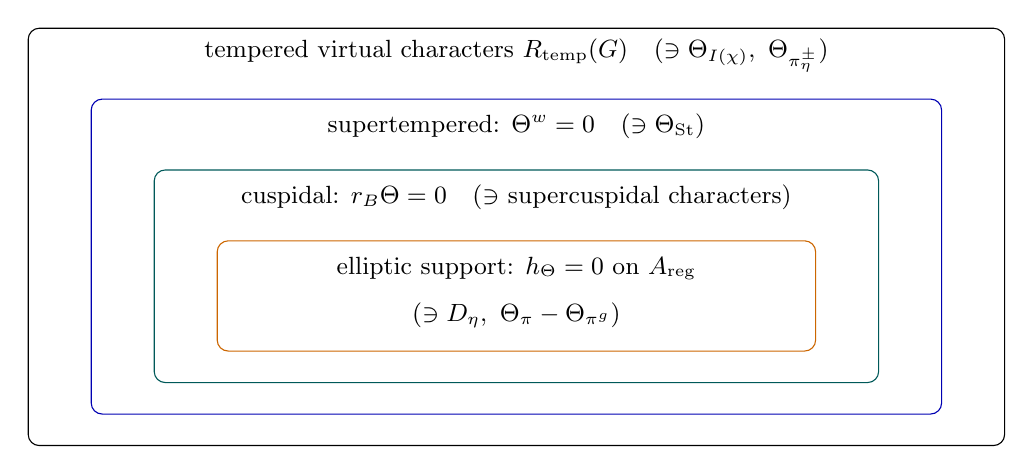
\begin{tikzpicture}[every node/.style={font=\small}]
\draw[rounded corners] (-6.2,-2.6) rectangle (6.2,2.7);
\node at (0,2.35) {tempered virtual characters $R_{\rm temp}(G)$\quad ($\ni\Theta_{I(\chi)},\ \Theta_{\pi_\eta^\pm}$)};
\draw[rounded corners,blue!70!black] (-5.4,-2.2) rectangle (5.4,1.8);
\node at (0,1.45) {supertempered: $\Theta^w=0$\quad ($\ni\Theta_{\St}$)};
\draw[rounded corners,teal!70!black] (-4.6,-1.8) rectangle (4.6,0.9);
\node at (0,.55) {cuspidal: $r_B\Theta=0$\quad ($\ni$ supercuspidal characters)};
\draw[rounded corners,orange!80!black] (-3.8,-1.4) rectangle (3.8,0);
\node at (0,-.35) {elliptic support: $h_\Theta=0$ on $A_{\rm reg}$};
\node at (0,-.95) {($\ni D_\eta,\ \Theta_{\pi}-\Theta_{\pi^g}$)};
\end{tikzpicture}
\caption{Four nested classes of tempered virtual characters. All inclusions are strict. Here $\pi^g$ is the conjugate of a depth-zero supercuspidal $\pi$ by $g=\operatorname{diag}(\varpi,1)$.}\label{fig:nested}
\end{figure}

\subsection{The quadratic constituents}\label{sub:quad}
The supertemperedness of $D_\eta$ has several proofs. Each shows something different, so the paper should give all of them.

\begin{theorem}\label{thm:Deta}\status{Proved}
Let $\eta$ be a nontrivial quadratic character and $E_\eta=F(\sqrt\tau)$ the corresponding quadratic extension.
\begin{enumerate}[label=(\alph*),leftmargin=*]
\item $D_\eta^w=0$ and $r_B(D_\eta)=0$.
\item $D_\eta=\tr\bigl(R(w,\eta)I(\eta)(\cdot)\bigr)$, where $R(w,\eta)$ is the normalized self-intertwining operator with $R(w,\eta)^2=1$.
\item $D_\eta\circ\operatorname{Ad}(x)=\eta(\det x)\,D_\eta$ for $x\in\mathrm{GL}_2(F)$.
\item $D_\eta(\gamma)=0$ for every regular semisimple $\gamma$ whose centralizer in $\mathrm{GL}_2(F)$ contains an element $x$ with $\eta(\det x)=-1$. This holds for all regular split $\gamma$ and for all regular elliptic $\gamma$ in tori that do not split over $E_\eta$.
\end{enumerate}
\end{theorem}
\begin{proof}
(a) is Table \ref{tab:four}. For (b), the commuting algebra of $I(\eta)$ has dimension two, by Frobenius reciprocity and $r_B\,I(\eta)=2\eta$, and it is spanned by $1$ and $R(w,\eta)$ \cite{Ke82}. The two constituents are the eigenspaces of $R(w,\eta)$ for $\pm1$. The operator acts on the two-dimensional Jacquet module with eigenvalues $+1$ and $-1$, so its trace there is zero. This is a second proof of (a).

(c) Section 8.4 of Draft 3 shows that $\mathrm{GL}_2(F)$ permutes $\{\pi_\eta^+,\pi_\eta^-\}$ transitively. The stabilizer of $\pi_\eta^+$ contains $\mathrm{SL}_2(F)$ and the center, and has index two. The irreducible principal series $I_{\mathrm{GL}_2}(\eta,1)$ is isomorphic to its twist by $\eta\circ\det$ and by no other nontrivial character of $F^\times/F^{\times2}$. By Clifford theory the stabilizer is the kernel of $\eta\circ\det$.

(d) Apply (c) with $x$ in the centralizer of $\gamma$. For split $\gamma=a(t)$ take $x=\operatorname{diag}(y,1)$ with $\eta(y)=-1$. For $\gamma$ in an elliptic torus attached to a quadratic extension $E'$, the centralizer is $E'^\times$ and $\det$ is the norm. If $E'\ne E_\eta$ then $\eta$ is nontrivial on the norms from $E'$.
\end{proof}
Part (d) is stronger than supertemperedness. It gives elliptic support, and it locates the support on the tori that split over $E_\eta$. This is the pattern of the Sally--Shalika formulas \cite{SS68} and of the endoscopic description of the packet $\{\pi_\eta^+,\pi_\eta^-\}$ \cite{LL79}. \status{Cited, memory}

For the unramified character $\eta_\varepsilon$ the values on the support can be computed by hand. Label the constituents so that $\pi_+$ has a $K_0$-fixed vector. Then $\pi_-$ has a $K_1$-fixed vector, by (c) with $x=\operatorname{diag}(\varpi,1)$. Let $X$ be the Bruhat--Tits tree. Its vertices have type $0$ or $1$ according to whether their stabilizer is conjugate in $G$ to $K_0$ or $K_1$. Adjacent vertices have different types. For a compact element $\gamma$ let $V_i(\gamma)$ be the number of fixed vertices of type $i$.

\begin{theorem}[Tree formula]\label{thm:tree}\status{Proved, given the Schneider--Stuhler character formula}
For every regular elliptic $\gamma$,
\[
\Theta_{\pi_\pm}(\gamma)=\pm\bigl(V_0(\gamma)-V_1(\gamma)\bigr),\qquad D_{\eta_\varepsilon}(\gamma)=2\bigl(V_0(\gamma)-V_1(\gamma)\bigr),\qquad \Theta_{\St}(\gamma)=-1 .
\]
If $\gamma$ lies in an unramified elliptic torus and its fixed set is the ball of radius $n$ around a vertex of type $i$, then $D_{\eta_\varepsilon}(\gamma)=2(-1)^i(-q)^n=2(-1)^{i+n}|\Delta_G(\gamma)|^{-1/2}$. If $\gamma$ lies in a ramified elliptic torus, then $D_{\eta_\varepsilon}(\gamma)=0$.
\end{theorem}
\begin{proof}
For a depth-zero representation $V$ and elliptic regular $\gamma$, Schneider and Stuhler prove
\[
\Theta_V(\gamma)=\sum_{x}\tr\bigl(\gamma\mid V^{K_x^+}\bigr)-\sum_{e}\tr\bigl(\gamma\mid V^{\mathcal I_e^+}\bigr),
\]
the sums running over the fixed vertices and fixed edges, with $K_x^+$ and $\mathcal I_e^+$ the pro-unipotent radicals \cite[Section III.4]{SS97}. \status{Cited, consulted through \cite{Ko04}; the level $e=0$ must be checked in the source} The space $I(\eta_\varepsilon)^{K_0^+}$ is the representation of $\mathrm{SL}_2(\mathbb F_q)$ induced from the trivial character of the Borel subgroup, which is $\triv\oplus\St_q$. Each of $\pi_\pm$ has a one-dimensional space of $\mathcal I$-fixed vectors. So $\pi_+^{K_x^+}$ is $\triv$ at vertices of type $0$ and $\St_q$ at vertices of type $1$, and $\pi_-$ is the reverse. Edge spaces are one-dimensional with trivial action. The value of $\St_q$ at the reduction of $\gamma$ at $x$ is the number of fixed points on $\mathbb P^1(\mathbb F_q)$ minus one, which is $\deg(x)-1$ with $\deg$ the degree in the fixed tree. Let $E$ be the number of fixed edges. Each edge has one endpoint of each type, so $\sum_{\text{type }1}\deg(x)=E$. Hence
\[
\Theta_{\pi_+}(\gamma)=V_0+(E-V_1)-E=V_0-V_1 .
\]
The same computation gives $\Theta_{\St}(\gamma)=\sum_x(\deg(x)-1)-E=E-(V_0+V_1)=-1$, the Euler characteristic of a finite tree with the sign reversed.

In a ball of radius $n$ around a vertex of type $i$ the sphere of radius $j\ge1$ has $(q+1)q^{j-1}$ vertices of type $i+j$. The alternating sum $1-(q+1)+(q+1)q-\cdots$ up to radius $n$ is $(-q)^n$. For such $\gamma$ one has $|\Delta_G(\gamma)|^{1/2}=q^{-n}$. A ramified elliptic element fixes a ball centered at the midpoint of an edge. Reflection in the midpoint is a bijection of that ball that exchanges types, so $V_0=V_1$.
\end{proof}
The two $G$-conjugacy classes of unramified elliptic tori are distinguished by the type $i$ of the vertex they fix, and $D_{\eta_\varepsilon}$ has opposite signs on them. The same method on a ball-truncated apartment, justified by Korman's theorem for compact elements in rank one \cite{Ko04}, gives $\Theta_{\St}(a(t))=2q^n-1$ and $\Theta_{\pi_\pm}(a(t))=q^n$ for $t\in1+\mathfrak p^n$, $t\notin 1+\mathfrak p^{n+1}$. These agree with the classical formulas, which checks the normalization.

\begin{proposition}[Explicit pseudo-coefficients]\label{prop:pseudo}\status{Proved}
Let $e_J=\vol(J)^{-1}\mathbf 1_J$. The functions
\[
f_-=e_{K_0}-e_{K_1},\qquad f_{\St}=e_{\mathcal I}-e_{K_0}-e_{K_1}
\]
have $f^{(B)}=0$. In the unramified block coordinates $(Q,d,b)$ of Section 5 they are $(0,2,0)$ and $(0,0,1)$, and their traces on all other blocks vanish. For elliptic regular $\gamma$ with $\vol(G_\gamma)=1$, $\mathcal O_\gamma(f_-)=V_0(\gamma)-V_1(\gamma)=\tfrac12D_{\eta_\varepsilon}(\gamma)$.
\end{proposition}
\begin{proof}
For unramified $\chi$, $\dim I(\chi)^{K_i}=1$ and $\dim I(\chi)^{\mathcal I}=2$. So both functions have trace zero on every $I(\chi)$, and by \eqref{eq:adj} and Mellin inversion $f^{(B)}=0$. Representations outside the unramified block have no $\mathcal I$-fixed vectors. The traces on $\pi_+,\pi_-,\St,\triv$ are $(1,-1,0,0)$ for $f_-$ and $(0,0,1,-1)$ for $f_{\St}$. The orbital integral of $e_{K_i}$ counts fixed vertices of type $i$.
\end{proof}
The function $-f_{\St}$ is Kottwitz's Euler--Poincar\'e function \cite{Ko88}. The formula for $\mathcal O_\gamma(f_-)$ is an instance of Kazhdan's orthogonality \cite{Ka86,SS97}, since $\|D_{\eta_\varepsilon}\|^2_{\rm ell}=4$ and $D_{\eta_\varepsilon}(f_-)=2$.

\subsection{The elliptic quotient and its two splittings}\label{sub:split}
This subsection answers the question left open at the end of Section 7 of Draft 3: what do the exceptional coordinates characterize?

Define two operators, the first on $R(G)$ and the second on $R_{\rm temp}(G)$:
\[
\mathsf A=1-\tfrac12\,i_B\,r_B,\qquad \mathsf A^w=1-\tfrac12\,i_B\,r_B^w .
\]
The first is the rank-one case of the operator used by Bernstein, Deligne and Kazhdan to isolate the elliptic part \cite{BDK86,Da00}. \status{Cited, memory, for the attribution only}

\begin{theorem}[Two complements of the induced part]\label{thm:twosplit}\status{Proved}
\begin{enumerate}[label=(\alph*),leftmargin=*]
\item $\mathsf A$ is idempotent with kernel $R_{\rm ind}(G)$. Its image $R_{\rm ell}(G)=\ker(i_Br_B)$ has basis the supercuspidal classes, the three $D_\eta$, and $\St-\triv$.
\item $\mathsf A^w$ is idempotent with kernel $R_{\rm ind}(G)\cap R_{\rm temp}(G)$ and image $\ST(G)$.
\item Both $R_{\rm ell}(G)$ and $\ST(G)$ map isomorphically onto the elliptic quotient $\overline R(G)$. The resulting isomorphism $\ST(G)\to R_{\rm ell}(G)$ is $\Theta\mapsto\mathsf A\Theta$. It is the identity on supercuspidal characters and on the $D_\eta$, and it sends $\St$ to $\tfrac12(\St-\triv)$.
\item For tempered $\Theta$ with Steinberg coefficient $\beta$, $\ \mathsf A^w\Theta-\mathsf A\Theta=\tfrac\beta2\,[I(|\cdot|)]$.
\end{enumerate}
\end{theorem}
\begin{proof}
In $R(A)$, $r_B\,i_B=1+w$, and $i_B\circ w=i_B$ in $R(G)$. So $\mathsf A\,i_B=i_B-\tfrac12(i_B+i_Bw)=0$ and $\mathsf A^2=\mathsf A-\tfrac12\mathsf A\,i_Br_B=\mathsf A$. The kernel is contained in the image of $i_B$ and contains it. The image is $\{x:i_Br_Bx=0\}$. Evaluating $\mathsf A$ on irreducibles gives $\mathsf A(\pi_\eta^\pm)=\pm\tfrac12D_\eta$, $\mathsf A(\St)=\tfrac12(\St-\triv)=-\mathsf A(\triv)$, $\mathsf A(\pi)=\pi$ for supercuspidal $\pi$, and $\mathsf A(I(\chi))=0$. This is (a). The same argument with $r_B^wi_B\chi=\chi+\chi^{-1}$ for unitary $\chi$ gives (b), and the image is $\ker r_B^w=\ST(G)$ by Theorem \ref{thm:herb}. Part (c) follows because both are complements of the same kernel. Part (d) is $\tfrac12i_B(r_B-r_B^w)\Theta$ and Table \ref{tab:four}.
\end{proof}

In the language of Sections 3 and 5 to 7 of Draft 3: the coordinate $b=\tr\St$ is the functional $\Theta_{\St}\in\ST(G)$, and the coordinate $d_{\St}=\tr\St-\tr\triv$ of Section 3 is the functional $2\mathsf A(\St)\in R_{\rm ell}(G)$. Both represent the same class modulo functionals of the induced trace $Q$, because $\Theta_{\triv}=\ev_c-\Theta_{\St}$. The phrase ``functionals with zero polynomial moments'' therefore depends on the coordinates chosen. With $(Q,d,b)$ it means $\ST$. With $(Q,d,d_{\St})$ it means $R_{\rm ell}$. With $(Q,d,t)$, $t=\tr\triv$, it would be the span of $D_\eta$ and the trivial character. Only the quotient is intrinsic. Temperedness selects $\ST$, and compatibility with Jacquet restriction selects $R_{\rm ell}$.

Now pass to functionals. For a Bernstein block $\mathfrak s$ let $\PW^{\mathfrak s}$ be the algebraic trace space of Section 5. Let $\PW^{\mathfrak s}_c$ be the subspace of trace forms vanishing on every $[I(\chi)]$, and $\PW^{\mathfrak s}_{\rm ind}=\PW^{\mathfrak s}/\PW^{\mathfrak s}_c$, the space of induced trace polynomials.

\begin{theorem}[Exact sequences and annihilators]\label{thm:exact}\status{Proved, given the block descriptions of Section 5}
For every block $\mathfrak s$ there are exact sequences, dual to each other,
\[
0\to\PW_c^{\mathfrak s}\to\PW^{\mathfrak s}\to\PW^{\mathfrak s}_{\rm ind}\to0,\qquad
0\to(\PW^{\mathfrak s}_{\rm ind})'\to(\PW^{\mathfrak s})'\to(\PW^{\mathfrak s}_c)'\to0 .
\]
The space $\PW_c^{\mathfrak s}$ is finite-dimensional and $(\PW_c^{\mathfrak s})'\simeq\overline R(G)^{\mathfrak s}$. Moreover:
\begin{enumerate}[label=(\alph*),leftmargin=*]
\item $(\PW^{\mathfrak s}_{\rm ind})'=\Ann(\PW^{\mathfrak s}_c)$. These are the functionals $D_L$ of Theorem 8.3 of Draft 3.
\item $(\PW^{\mathfrak s})'=(\PW^{\mathfrak s}_{\rm ind})'\oplus\ST^{\mathfrak s}$, and $\ST^{\mathfrak s}=\Ann(N^{\mathfrak s}_{\rm temp})$, where $N^{\mathfrak s}_{\rm temp}$ is the space of trace forms $\pi\mapsto\tfrac12\psi(r_B^w\pi)$ on tempered $\pi$, with $\psi$ a Weyl-invariant regular function on the twist torus. In the unramified block $N_{\rm temp}=\{(Q,0,0)\}$.
\item $(\PW^{\mathfrak s})'=(\PW^{\mathfrak s}_{\rm ind})'\oplus R^{\mathfrak s}_{\rm ell}$, and $R_{\rm ell}^{\mathfrak s}=\Ann(N^{\mathfrak s}_{\rm alg})$, where $N^{\mathfrak s}_{\rm alg}$ is the space of trace forms $\pi\mapsto\tfrac12\psi(r_B\pi)$. In the unramified block $N_{\rm alg}=\{(Q,0,\tfrac12Q(c))\}$.
\end{enumerate}
\begin{center}\small
\begin{tabular}{@{}lcccl@{}}\toprule
Block & $\PW_{\rm ind}^{\mathfrak s}$ & $\dim\PW_c^{\mathfrak s}$ & isolated points of $T_{\mathfrak s}/\!/W_{\mathfrak s}$ & basis of $\ST^{\mathfrak s}$\\\midrule
supercuspidal & $0$ & $1$ & $1$ & $\Theta_\pi$\\
I, $\xi^2\ne1$ & $\mathbb C[z,z^{-1}]$ & $0$ & $0$ & none\\
II, $\xi^2=1\ne\xi$ & $\mathbb C[u]$ & $2$ & $2$ & $D_\eta$ at $z=1$ and at $z=-1$\\
III, $\xi=1$ & $\mathbb C[u]$ & $2$ & $2$ & $D_{\eta_\varepsilon}$, $\Theta_{\St}$\\\bottomrule
\end{tabular}
\end{center}
\end{theorem}
\begin{proof}
Exactness is the definition. In coordinates, $\PW_c$ is $\{Q=0\}$, and $N_{\rm temp}$, $N_{\rm alg}$ are complements of it, as one sees by evaluating $\tfrac12\psi\circ r_B^w$ and $\tfrac12\psi\circ r_B$ on $\pi_\pm$, $\St$, $\triv$ with Table \ref{tab:four}. The annihilator of a complement of $\PW_c$ is a complement of $\Ann(\PW_c)$ that maps isomorphically to $(\PW_c)'$. The functionals $d$ and $b$ vanish on $N_{\rm temp}$, and $d$ and $2b-\ev_c$ vanish on $N_{\rm alg}$.
\end{proof}
So supertempered characters are annihilators of induced trace data, in a precise sense: they kill the trace forms that factor through the weak Jacquet functor. The extended quotient of Section 3 counts them. In Type II both isolated points carry a nontrivial $R$-group. In Type III the point $e_-$ carries $D_{\eta_\varepsilon}$, and the point $e_+$ at $z=1$, where the $R$-group is trivial, carries Steinberg after the correcting cocharacter moves its support to $c$. The count $4=1+3$ of Corollary \ref{cor:irr} is also the number of elliptic endoscopic data of $\mathrm{SL}_2$: the group itself and the three norm-one tori \cite{LL79}.

\begin{figure}[htbp]\centering
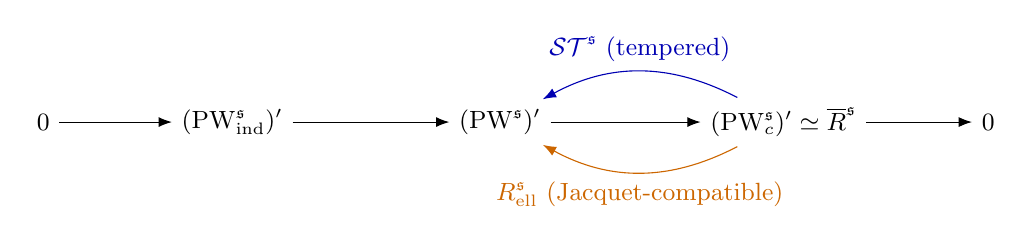
\begin{tikzpicture}[>=Latex,every node/.style={font=\small}]
\node (a) at (0,0) {$0$};
\node (b) at (2.4,0) {$(\PW_{\rm ind}^{\mathfrak s})'$};
\node (c) at (5.8,0) {$(\PW^{\mathfrak s})'$};
\node (d) at (9.4,0) {$(\PW_c^{\mathfrak s})'\simeq\overline R^{\mathfrak s}$};
\node (e) at (12,0) {$0$};
\draw[->] (a)--(b);\draw[->] (b)--(c);\draw[->] (c)--(d);\draw[->] (d)--(e);
\draw[->,blue!70!black,bend right=28] (d) to node[above] {$\ST^{\mathfrak s}$ (tempered)} (c);
\draw[->,orange!80!black,bend left=28] (d) to node[below] {$R^{\mathfrak s}_{\rm ell}$ (Jacquet-compatible)} (c);
\end{tikzpicture}
\caption{One quotient, two splittings. Their difference is $\beta\mapsto\frac\beta2\ev_c$ on the Steinberg line and zero elsewhere.}\label{fig:splittings}
\end{figure}

\subsection{The weak constant term of a distribution}\label{sub:wct}
Herb defines weak constant terms for virtual characters. Section 8 of Draft 3 treats arbitrary spectral functionals. The two meet as follows. Let $D$ be an invariant distribution supported in a principal series block with unit character $\xi$. By Theorem \ref{thm:exact}(b) write $D=D_L+\Theta^{\rm st}$ uniquely, with $L$ a functional on the induced trace polynomial and $\Theta^{\rm st}\in\ST^{\mathfrak s}$.

\begin{definition}\label{def:wct}
The \emph{weak constant term} of $D$ is the function on $A$
\[
D^w_B(a(t))=L\bigl(z\mapsto\chi_{\xi,z}(t)+\chi_{\xi,z}(t)^{-1}\bigr).
\]
In the unramified block, with $m_n=L(B_n)$, this is $m_{|v(t)|}$ for $v(t)\ne0$ and $2m_0$ on $A^0$.
\end{definition}

\begin{theorem}[Canonical decomposition]\label{thm:decomp}\status{Proved; part (e) Conditional}
\begin{enumerate}[label=(\alph*),leftmargin=*]
\item $D^w_B$ is a Weyl-invariant locally constant function on all of $A$, including $\pm I$.
\item For every $f\in C_c^\infty(G)$, $\ D(f)=\tfrac12\int_AD^w_B(a)\,f^{(B)}(a)\,da+\Theta^{\rm st}(f)$.
\item If $D$ is a tempered virtual character, $D^w_B$ is Herb's weak constant term.
\item On $A_{\rm reg}$, $h_D=D^w_B+h_{\Theta^{\rm st}}$, and $h_{\Theta^{\rm st}}(a(t))=\beta q^{-|v(t)|}$ for $v(t)\ne0$.
\item In the smooth model of Section 6, $D$ is tempered if and only if $|D^w_B(a(t))|\le C(1+|v(t)|)^N$.
\item $D^w_B=0$ if and only if $D\in\ST^{\mathfrak s}$.
\end{enumerate}
\end{theorem}
\begin{proof}
(a) is Theorem 8.6 of Draft 3. For (b), $f^{(B)}$ is locally constant with compact support, so the integral in \eqref{eq:adj} is a finite sum of terms $\chi_{\xi,z}(a_j)c_j$, and $L$ may be applied term by term. For (c) take $L=\ev_{z_0}$ and use Table \ref{tab:four}, with $\pi_\eta^\pm=\tfrac12I(\eta)\pm\tfrac12D_\eta$. Part (d) is Theorem 8.3 of Draft 3 together with Proposition \ref{prop:bohr}. Part (e) is Theorem 6.1 of Draft 3. Part (f) holds because $L$ is determined by its moments.
\end{proof}
Thus the corrected descent theorem of Section 8 is a statement about weak constant terms: the weak constant term of a finite-block distribution is an admissible distribution on $A$, and the distribution is supertempered when it vanishes. For a non-tempered virtual character the same formula gives its induced part relative to the tempered splitting. For example $\Theta_{\triv}$ has $D^w_B=|t|+|t|^{-1}$ and $\Theta^{\rm st}=-\Theta_{\St}$.

\subsection{Singular behavior at $\pm I$}\label{sub:germ}
The weak constant term sees only infinity. Near $\pm I$ a different invariant governs, and it is not zero for supertempered characters.

\begin{theorem}[Split germ at the identity]\label{thm:germ}\status{Proved from the local character expansion, which is Cited, memory}
For every $\Theta\in R(G)$ there are constants $w(\Theta)$ and $c_0(\Theta)$ and a neighborhood of $1$ in $F^\times$ on which
\[
h_\Theta(a(t))=\tfrac12\,w(\Theta)+c_0(\Theta)\,|t-t^{-1}|\qquad(t\ne1).
\]
Here $c_0(\Theta)$ is the coefficient of the trivial nilpotent orbit in the Harish-Chandra--Howe expansion, and $w(\Theta)=\sum_{\mathcal O}c_{\mathcal O}(\Theta)$ is the sum over the four regular nilpotent orbits. For irreducible $\pi$, $h_\pi(-a(t))=\omega_\pi(-1)h_\pi(a(t))$ gives the expansion at $-I$.
\end{theorem}
\begin{proof}
Near the identity $\Theta(\exp X)=c_0+\sum_{\mathcal O}c_{\mathcal O}\widehat\mu_{\mathcal O}(X)$ \cite{HC99}. For a regular nilpotent orbit, $\widehat\mu_{\mathcal O}(sX)=|s|^{-1}\widehat\mu_{s\mathcal O}(X)$. Conjugation by $\operatorname{diag}(1,s)$ fixes the split element $X_x=\operatorname{diag}(x,-x)$, preserves the invariant form, and permutes the four regular orbits transitively. So the four functions $\widehat\mu_{\mathcal O}$ agree on the split Cartan subalgebra, and $\widehat\mu_{\mathcal O}(X_{sx})=|s|^{-1}\widehat\mu_{\mathcal O}(X_x)$ for all $s$. Hence $\widehat\mu_{\mathcal O}(X_x)=\kappa/|2x|$ with one constant $\kappa$. The case $\Theta=\Theta_{I(\chi)}$, where $h=\chi+\chi^{-1}\to2$ and all four coefficients are $1$, gives $\kappa=\tfrac12$.
\end{proof}

\begin{center}\small
\begin{tabular}{@{}lccl@{}}\toprule
$\pi$ & $w(\pi)$ & $c_0(\pi)$ & source of the values\\\midrule
$I(\chi)$ irreducible & $4$ & $0$ & character formula\\
$\pi_\eta^\pm$ & $2$ & $0$ & $h=\eta$\\
$\St$ & $4$ & $-1$ & $h=2-|t-t^{-1}|$\\
$\triv$ & $0$ & $1$ & $h=|t-t^{-1}|$\\
discrete series $\pi$ & $1$, $2$ or $4$ & $-d(\pi)/d(\St)$ & Harish-Chandra; Rodier\\\bottomrule
\end{tabular}
\end{center}
By Rodier's theorem $w(\pi)$ is the number of classes $a\in F^\times/F^{\times2}$ for which $\pi$ has a Whittaker model with respect to $\psi_a$ \cite{Ro75}. The formula $c_0(\pi)=-d(\pi)/d(\St)$ for the discrete series is Harish-Chandra's \cite{HC99}. \status{Cited, memory} With $\vol(K_0)=1$ the Euler--Poincar\'e measure gives $d(\St)=q-1$. Both are confirmed independently by the next proposition.

\begin{proposition}[A depth-zero supercuspidal character on the split torus]\label{prop:sc}\status{Proved, given Korman's theorem \cite{Ko04}}
Let $\sigma$ be a cuspidal representation of $\mathrm{SL}_2(\mathbb F_q)$ of dimension $q-1$, inflated to $K_0$, and $\pi=\operatorname{c-Ind}_{K_0}^G\sigma$. For $t\in\mathcal O^\times$, $t\ne\pm1$,
\[
\Theta_\pi(a(t))=\begin{cases}\omega_\pi(\pm1)\bigl(|t-t^{-1}|^{-1}-1\bigr),&t\in\pm(1+\mathfrak p),\\ 0,&t\not\equiv\pm1\bmod\mathfrak p,\end{cases}
\]
and $\Theta_\pi(a(t))=0$ for $|t|\ne1$. So $w(\pi)=2$ and $c_0(\pi)=-1=-d(\pi)/d(\St)$. The same formula holds for the sum of the two cuspidal representations of dimension $(q-1)/2$.
\end{proposition}
\begin{proof}
Only vertices of type $0$ contribute, with $\pi^{K_x^+}\simeq\sigma$, and edges contribute nothing because $\sigma$ has no vector fixed by the unipotent radical. Let $t\in1+\mathfrak p^n$, $t\notin1+\mathfrak p^{n+1}$. The fixed set of $a(t)$ is the set of vertices at distance at most $n$ from the standard apartment. At distance $j<n$ the element reduces to the identity, with trace $q-1$. At distance $n$ it reduces to a nontrivial unipotent, with trace $-1$. There are $(q-1)q^{j-1}$ vertices at distance $j\ge1$ over each apartment vertex, and the type is the parity of position plus distance. Truncate at the ball of radius $R$ around a vertex of the apartment. A pair of adjacent complete columns contributes zero. The incomplete columns at the two ends contribute a total that is independent of $R$, and the sum is $q^n-1$. For $t\not\equiv\pm1$ the fixed set is the apartment and the trace of $\sigma$ at a regular split element is zero. The case $|t|\ne1$ is Proposition \ref{prop:cass}.
\end{proof}
I verified the sum $q^n-1$, and the corresponding values $2q^n-1$ for Steinberg and $1$ for the trivial representation, exactly for $q\in\{3,5,7\}$, $n\le4$ and several $R$. These values should still be compared with the tables of \cite{SS68,ADSS11}, which I did not consult.

\begin{corollary}[Split descent criterion]\label{cor:descent}\status{Proved, given Theorem \ref{thm:germ}}
Let $\Theta=\sum a_\pi\Theta_\pi$ be a virtual character. Its normalized split restriction extends to a locally constant function on all of $A$ if and only if
\[
\sum_\pi a_\pi\,c_0(\pi)=0\quad\text{and}\quad\sum_\pi a_\pi\,\omega_\pi(-1)\,c_0(\pi)=0 .
\]
For supertempered $\Theta$ this reads $\sum a_\pi\,\omega_\pi(\pm1)\,d(\pi)=0$, the sums over the discrete series. For an invariant distribution with finite Bernstein support the criterion applies to its part $\Theta^{\rm st}$, because the induced part always descends (Theorem \ref{thm:decomp}(a)).
\end{corollary}
Within the unramified block the criterion is $\beta=0$, which is Theorem 8.8 of Draft 3. Across blocks the Steinberg obstruction can cancel.
\begin{example}[Steinberg minus a supercuspidal]\label{ex:cancel}
Let $F=\mathbb Q_5$ and let $\theta$ be a character of order three of the group $\mu_6$ of norm-one elements of $\mathbb F_{25}$. Then $\theta(-1)=1$, the cuspidal representation $\sigma_\theta$ has dimension $4$, and $\pi=\operatorname{c-Ind}\sigma_\theta$ has $\omega_\pi(-1)=1$. By Table \ref{tab:four}, $\Theta_{\St}-\Theta_\pi$ has
\[
h(a(t))=5^{-|v(t)|}\quad\text{for all regular }t .
\]
It is locally constant across $\pm I$ although the Steinberg coefficient is $1$. Over $\mathbb Q_3$ the only cuspidal representation of dimension $q-1=2$ has $\omega(-1)=-1$. There one uses $\Theta_{\St}-\Theta_{\pi_0^+}-\Theta_{\pi_0^-}$, with $\pi_0^\pm$ induced from the two nontrivial one-dimensional characters of $\mathrm{SL}_2(\mathbb F_3)$, and obtains $h(a(t))=3^{-|v(t)|}$.
\end{example}
\begin{figure}[htbp]\centering
\begin{tikzpicture}[x=1.3cm,y=1.6cm,>=Latex,every node/.style={font=\small}]
\draw[->] (0.5,0)--(6.8,0) node[right]{$n$};
\draw[->] (0.5,0)--(0.5,2.35) node[above]{$h(a(1+5^n))$};
\foreach \y in {1,2}{\draw (0.42,\y)--(0.58,\y) node[left,xshift=-4pt]{\y};}
\foreach \n/\s in {1/0.2,2/0.04,3/0.008,4/0.0016,5/0.0003,6/0.0001}{
\fill[blue!70!black] (\n,{2-\s}) circle (1.6pt);
\fill[teal!70!black] (\n,{1-\s}) circle (1.6pt);
\draw[orange!80!black,thick] (\n-0.08,1.03)--(\n+0.08,1.03);
\node[below] at (\n,0) {\n};}
\node[blue!70!black,anchor=west] at (2.3,2.17) {$\St$: $2-5^{-n}$};
\node[teal!70!black,anchor=west] at (2.3,0.72) {$\pi$: $1-5^{-n}$};
\node[orange!80!black,anchor=west] at (2.3,1.25) {$\St-\pi$: constant $1$};
\end{tikzpicture}
\caption{Normalized split restrictions along $t=1+5^n$ in $\mathbb Q_5$. Each discrete series character fails to be locally constant at $I$. The difference is constant.}\label{fig:cancel}
\end{figure}

\subsection{The Bernstein center and Hecke-finiteness}\label{sub:center}
Section 7 of Draft 3 classifies central eigenfunctionals and jets. Three consequences bear on supertemperedness.

\begin{proposition}\label{prop:center}\status{Proved, given Theorems 7.2 and 7.3 of Draft 3}
\begin{enumerate}[label=(\alph*),leftmargin=*]
\item An invariant distribution with finite Bernstein support is a virtual character if and only if it is a finite sum of eigendistributions of the Bernstein center. It is center-finite if and only if it is a finite sum of jets $\partial_\theta^j\Theta_{I(\chi_\theta)}$ and irreducible characters.
\item Every supertempered virtual character is a finite sum of central eigendistributions. In a principal series block the eigencharacters lie in the finite set of doubled support points.
\item The center cannot detect supertemperedness. At $u=-2$ the eigenspace is spanned by $D_\eta$ and $\Theta_{I(\eta)}$, and at $u=c$ by $\Theta_{\St}$ and $\Theta_{\triv}$. In each pair exactly one element is supertempered.
\item A center-finite tempered distribution with $D^w_B=0$ is a supertempered virtual character.
\end{enumerate}
\end{proposition}
\begin{proof}
(a) The eigenspace at a generic point is the line of $\ev_\mu=\Theta_{I(\chi)}$, and at an exceptional point it is the span of the two irreducible characters of the fiber. The generalized eigenspaces are described by Theorem 7.3. (b) and (c) are read off from Corollary \ref{cor:irr}. (d) A jet of order $j$ at a unitary point has $D^w_B(a(t))$ equal to $v(t)^j$ times a nonzero almost periodic function, and distinct jets are independent. So $D^w_B=0$ forces the jet part to vanish.
\end{proof}

\begin{proposition}[Hecke-finite and center-finite]\label{prop:hecke}
\status{Proved in outline} Let $D$ be an invariant distribution. With the definition of the 1994 notes, taken from \cite[Section 1.10]{Si79}, $D$ is Hecke-finite if and only if each of its block components is center-finite. In particular:
\begin{enumerate}[label=(\alph*),leftmargin=*]
\item The jet $\partial_\theta\Theta_{I(\chi_\theta)}$ at a generic unitary point is Hecke-finite and is not a virtual character.
\item A locally finite infinite sum such as $\sum_\pi d(\pi)\Theta_\pi$ over all supercuspidals is Hecke-finite and is not a virtual character.
\end{enumerate}
\end{proposition}
\begin{proof}[Outline]
In the compact picture, $D_f(x)=\partial_\theta\tr\bigl(I_\theta(f)I_\theta(x^{-1})\bigr)$ lies in the finite-dimensional space of functions $\tr(B\,I_\theta(x^{-1}))+\tr(B'\,\partial_\theta I_\theta(x^{-1}))$ with $B,B'$ endomorphisms of a fixed space of $K'$-fixed vectors. That space is stable under right convolution by $C_c(G/\!/K)$. This gives (a) and, with higher derivatives, the ``if'' direction. Conversely, the fixed-level Hecke algebra contains the block center cut down by its idempotent. Hecke-finiteness of $D_f$ gives a polynomial $p_f$ in the central coordinate that kills the corresponding translates. The block of the cocenter is finitely generated over the block center, so finitely many $f$ suffice and their product kills the block component. For (b), each $f$ has nonzero trace on finitely many supercuspidals.
\end{proof}
So the 1994 lemma ``a Hecke-finite distribution is a virtual character'' is false as stated. The correct statement is Proposition \ref{prop:center}(a) with finite support added. The 1994 corollary ``a supertempered distribution is a virtual character'' is true for finite Bernstein support, by Proposition \ref{prop:center}(d). Draft 3 says that Hecke-finiteness ``is not a synonym for center-finiteness.'' In rank one, with Silberger's definition, it is a synonym block by block.

\begin{remark}[Infinite support]\label{rem:infinite}\status{Heuristic}
The distribution $\delta_{\rm cusp}=\sum_\pi d(\pi)\Theta_\pi$, the supercuspidal part of the Plancherel formula for $\delta_I$, is tempered, is Hecke-finite, and has zero weak constant term in every block. A count of supercuspidals by depth suggests $\delta_{\rm cusp}(e_{K_m})\ge c\,\vol(K_m)^{-1}$ with $c>0$. If so, it is not locally integrable and not admissible. This would show that the chain ``Hecke-finite, hence virtual character, hence admissible'' of the 1994 notes needs finite Bernstein support at both steps.
\end{remark}

\subsection{Euler--Poincar\'e pairings and the infinite dihedral Hecke algebra}\label{sub:EP}
The elliptic quotient carries the Euler--Poincar\'e form $\EP(\pi,\pi')=\sum_i(-1)^i\dim\Ext^i_G(\pi,\pi')$. It equals the elliptic inner product of characters \cite{Ka86,SS97} and is given on tempered representations by Arthur's $R$-group formula \cite{Ar93,OS13}. \status{Cited, consulted for the statements} In a quadratic block it can be computed by hand.

The unramified block is equivalent to the modules over the Iwahori--Hecke algebra $\mathcal H$ \cite{Bo76}. That algebra is generated by $T_0,T_1$ with the relations $(T_i-q)(T_i+1)=0$ and no others, because the affine Weyl group is the infinite dihedral group $\mathbb Z/2*\mathbb Z/2$. It has four characters $(\epsilon_0,\epsilon_1)$ with $\epsilon_i\in\{q,-1\}$:
\[
\triv=(q,q),\qquad\St=(-1,-1),\qquad\pi_+=(q,-1),\qquad\pi_-=(-1,q).
\]
A Type II block is equivalent to modules over the same algebra with $q$ replaced by $1$, the group algebra of $\mathbb Z/2*\mathbb Z/2$ \cite{Ro98}. \status{Cited, memory} Its four characters are the four constituents at $z=\pm1$.

\begin{proposition}\label{prop:EP}\status{Proved, given the equivalences of categories}
Write $\mathcal H=\mathcal H_0*\mathcal H_1$, with $\mathcal H_i$ generated by $T_i$. For finite-dimensional $\mathcal H$-modules $M$ and $N$,
\[
\EP(M,N)=\dim\Hom_{\mathcal H_0}(M,N)+\dim\Hom_{\mathcal H_1}(M,N)-\dim M\cdot\dim N .
\]
For two characters, $\EP=[\epsilon_0=\epsilon_0']+[\epsilon_1=\epsilon_1']-1$. On $(\triv,\St,\pi_+,\pi_-)$ the Gram matrix is
\[
\begin{pmatrix}1&-1&0&0\\-1&1&0&0\\0&0&1&-1\\0&0&-1&1\end{pmatrix}.
\]
Its radical is spanned by $[\triv]+[\St]$ and $[\pi_+]+[\pi_-]$, the two induced classes. The classes of $\St$ and $\pi_+$ form an orthonormal basis of the elliptic quotient of the block, and $\EP(D_\eta,D_\eta)=4$.
\end{proposition}
\begin{proof}
For a free product of two semisimple algebras there is a Mayer--Vietoris sequence $0\to\Hom_{\mathcal H}\to\Hom_{\mathcal H_0}\oplus\Hom_{\mathcal H_1}\to\Hom_{\mathbb C}\to\Ext^1_{\mathcal H}\to0$, and the higher groups vanish. It is the algebraic form of the action on the tree, with vertex stabilizers $K_0,K_1$ and edge stabilizer $\mathcal I$. The rest is counting.
\end{proof}
The formula is the trace of Kottwitz's function in disguise, and it reproduces Arthur's formula: for the two characters $\pm1$ of the $R$-group $\mathbb Z/2$, $|R|^{-1}|d(w)|(\pm1)(\pm1)=\pm1$ with $d(w)=\det(1-w)=2$. It also gives $\Ext^1(\pi_+,\pi_-)\simeq\mathbb C$ and $\Ext^1(\pi_\pm,\pi_\pm)=0$.

\begin{figure}[htbp]\centering
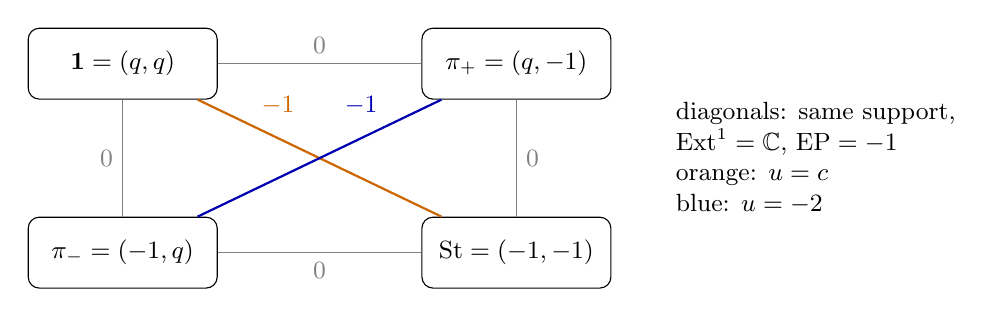
\begin{tikzpicture}[every node/.style={font=\small},>=Latex]
\node[draw,rounded corners,minimum width=2.4cm,minimum height=9mm] (t) at (0,2.4) {$\triv=(q,q)$};
\node[draw,rounded corners,minimum width=2.4cm,minimum height=9mm] (p) at (5,2.4) {$\pi_+=(q,-1)$};
\node[draw,rounded corners,minimum width=2.4cm,minimum height=9mm] (m) at (0,0) {$\pi_-=(-1,q)$};
\node[draw,rounded corners,minimum width=2.4cm,minimum height=9mm] (s) at (5,0) {$\St=(-1,-1)$};
\draw[gray] (t)--node[above]{$0$}(p);\draw[gray] (t)--node[left]{$0$}(m);
\draw[gray] (p)--node[right]{$0$}(s);\draw[gray] (m)--node[below]{$0$}(s);
\draw[thick,orange!80!black] (t)--node[pos=.22,above right]{$-1$}(s);
\draw[thick,blue!70!black] (p)--node[pos=.22,above left]{$-1$}(m);
\node[anchor=west,align=left] at (6.9,1.2) {diagonals: same support,\\ $\Ext^1=\mathbb C$, $\EP=-1$\\ orange: $u=c$\\ blue: $u=-2$};
\end{tikzpicture}
\caption{The four characters of the Hecke algebra of a quadratic block and their Euler--Poincar\'e pairings. Each has $\EP$ equal to $1$ with itself. Characters that differ in one coordinate are orthogonal. The two diagonals are the doubled fibers of the support map.}\label{fig:grid}
\end{figure}

\begin{example}[The elliptic norm of Steinberg by direct integration]\label{ex:norm}\status{Proved}
Since $\Theta_{\St}=-1$ on the elliptic set, $\EP(\St,\St)=1$ is the identity $\sum_T|W_T|^{-1}\int_T|\Delta_G(t)|\,dt=1$, with each elliptic torus of volume one. The two classes of unramified tori together contribute $(q^2-q+1)/(q^2+q+1)$. Each ramified quadratic extension contributes $q/(q^2+q+1)$. The total is $1$. For $\mathbb Q_3$ the three terms are $7/13,3/13,3/13$. For $\mathbb Q_5$ they are $21/31,5/31,5/31$. In the same way $|\Delta_G|\,|D_\eta|^2=4$ on the tori that split over $E_\eta$ gives $\|D_\eta\|^2_{\rm ell}=4$.
\end{example}
For the unramified computation, the norm-one group of $E$ maps onto the $q+1$ norm-one elements of the residue field, $|\Delta_G|=1$ off the classes of $\pm1$, and $|\Delta_G|=q^{-2n}$ on a shell of measure $(q-1)/((q+1)q^n)$ around each of $\pm1$. For a ramified extension, the Cayley parametrization $\lambda=\pm(1+y\sqrt\varpi)/(1-y\sqrt\varpi)$, $y\in\mathcal O$, gives $|\Delta_G|=q^{-2k-1}$ on the shell $v(y)=k$.

Later literature places these facts in a general theory: elliptic representations of Weyl groups \cite{Re01}, the elliptic and rigid cocenters \cite{CH17,CH21}, and extensions of tempered representations \cite{OS13}. \status{Cited, consulted for titles and abstracts only} In that language $\dim\ST^{\mathfrak s}=2$ is the number of elliptic conjugacy classes of $\mathbb Z/2*\mathbb Z/2$, the two classes of reflections.

\subsection{Examples and counterexamples over $\mathbb Q_3$ and $\mathbb Q_5$}\label{sub:counter}
\begin{center}\small
\begin{tabular}{@{}p{.36\linewidth}p{.27\linewidth}p{.27\linewidth}@{}}\toprule
Quantity & $F=\mathbb Q_3$ & $F=\mathbb Q_5$\\\midrule
$c=q+q^{-1}$ & $10/3$ & $26/5$\\
Quadratic characters & $\eta_2$ unramified, $\eta_3,\eta_6$ & $\eta_2$ unramified, $\eta_5,\eta_{10}$\\
Ramified quadratic block: $z=+1$, $z=-1$ & $\eta_6$, $\eta_3$ & $\eta_5$, $\eta_{10}$\\
Is $-1$ a square? & no & yes\\
Classes of elliptic tori & $2+1+1=4$ & $2+2+2=6$\\
$\Theta_{\St}(a(1+p^n))=2q^n-1$ & $5,17,53$ & $9,49,249$\\
$D_{\eta_2}$ on unramified tori, radius $n$ & $\pm2,\mp6,\pm18$ & $\pm2,\mp10,\pm50$\\
Depth-zero supercuspidals & $6$ & $8$\\
$d(\St)$, with $\vol(K_0)=1$ & $2$ & $4$\\
Example \ref{ex:cancel} & $\St-\pi_0^+-\pi_0^-$ & $\St-\pi(\theta)$, $\theta^3=1$\\\bottomrule
\end{tabular}
\end{center}
The second and third rows use $(3,3)_3=-1$, $(3,2)_3=-1$, $(5,5)_5=1$ and $(5,2)_5=-1$. When $-1$ is not a norm from a ramified extension, the two rational classes in a ramified torus are exchanged by the Weyl element, so there is one class of tori with trivial rational Weyl group.

The false implications, each with a witness:
\begin{enumerate}[leftmargin=*]
\item \emph{Supertempered does not imply cuspidal.} Steinberg: $J_{\St}=|t|$.
\item \emph{Cuspidal does not imply elliptic support.} A depth-zero supercuspidal: over $\mathbb Q_5$, $\Theta_{\pi(\theta)}(a(1+5^n))=5^n-1$.
\item \emph{Elliptic support does not imply ``in the span of the $D_\eta$.''} For a depth-zero supercuspidal $\pi$, the difference $\Theta_\pi-\Theta_{\pi^g}$ with $g=\operatorname{diag}(\varpi,1)$ vanishes on the split set because $g$ commutes with $A$. It is nonzero because $\pi^g$ has its type on $K_1$.
\item \emph{Elliptic representation does not imply supertempered character.} $\pi_\eta^+$.
\item \emph{An elliptic class need not have a tempered Jacquet-compatible representative.} $\tfrac12(\St-\triv)$.
\item \emph{Zero weak constant term does not imply local constancy of the split restriction}, and local constancy does not imply $\beta=0$. Steinberg, and Example \ref{ex:cancel}.
\item \emph{Tempered with vanishing regular density does not imply supertempered.} $\delta_I$ vanishes on the regular set, and its weak constant term in each block is the Plancherel density.
\item \emph{Decay of $h_D$ does not imply supertempered, outside virtual characters.} Take a wave packet $\int\Theta_{I(\chi_z)}g(z)\,dz$ with $g$ smooth. Its $h$ is given by the Fourier coefficients of $g$, which decay rapidly, and it is purely induced.
\item \emph{Elliptic support does not imply supertempered, outside virtual characters.} See the next example.
\end{enumerate}

\begin{example}[An elliptically supported distribution that is not supertempered]\label{ex:poisson}\status{Proved, given Proposition \ref{prop:sc}}
Let $F=\mathbb Q_5$ and $\pi=\pi(\theta)$ as in Example \ref{ex:cancel}. Let\[P(\vartheta)=\tfrac12+\sum_{n\ge1}q^{-n}\cos n\vartheta,\qquad L_P(Q)=\frac1{2\pi}\int_0^{2\pi}Q(2\cos\vartheta)P(\vartheta)\,d\vartheta .\]The function $P$ is a Poisson kernel. The moments of $L_P$ are $m_0=\tfrac12$ and $m_n=q^{-n}$. Put
\[
D=\Theta_{\St}-\Theta_\pi-D_{L_P}.
\]
By Example \ref{ex:cancel} and Theorem \ref{thm:decomp}(d) the normalized split restriction of $D$ is $q^{-|v(t)|}-q^{-|v(t)|}=0$ on all of $A_{\rm reg}$. So $D$ has elliptic support. It is invariant, has finite Bernstein support, is admissible by Theorem 8.5 of Draft 3, and is tempered in the smooth model. It is not supertempered: $D^w_B(a(t))=-q^{-|v(t)|}\ne0$. On the elliptic set $D=-1-\Theta_\pi$, so $D\ne0$. Over $\mathbb Q_3$ replace $\pi$ by $\pi_0^+\oplus\pi_0^-$.
\end{example}
The example shows that Hecke-finiteness is essential in the 1994 lemma (Corollary \ref{cor:1994}(c)). It also shows that elliptic support is not a spectral condition on one block.

\subsection{A global characterization}\label{sub:global}
\begin{theorem}\label{thm:global}\status{Proved from the results above; (b) Conditional; (a) uses the inputs of Theorem 8.5 of Draft 3}
Let $D$ be an invariant distribution on $G$ with finite Bernstein support. Write $D=\sum_{\mathfrak s}D_{L_{\mathfrak s}}+\Theta^{\rm st}$ with $\Theta^{\rm st}\in\ST(G)$.
\begin{enumerate}[label=(\alph*),leftmargin=*]
\item $D$ is admissible and locally representable.
\item $D$ is tempered if and only if every $L_{\mathfrak s}$ has polynomially bounded moments.
\item $D$ is center-finite if and only if every $L_{\mathfrak s}$ is a finite combination of jets, and a virtual character if and only if every $L_{\mathfrak s}$ is a finite combination of evaluations.
\item $D$ is supertempered, in the sense $D^w_B=0$, if and only if every $L_{\mathfrak s}=0$. Then $D$ is a virtual character.
\item $D$ is cuspidal if and only if in addition the Steinberg coefficient of $\Theta^{\rm st}$ is zero.
\item The normalized split restriction of $D$ is locally constant on $A$ if and only if $\Theta^{\rm st}$ satisfies Corollary \ref{cor:descent}.
\end{enumerate}
\end{theorem}
\begin{figure}[htbp]\centering
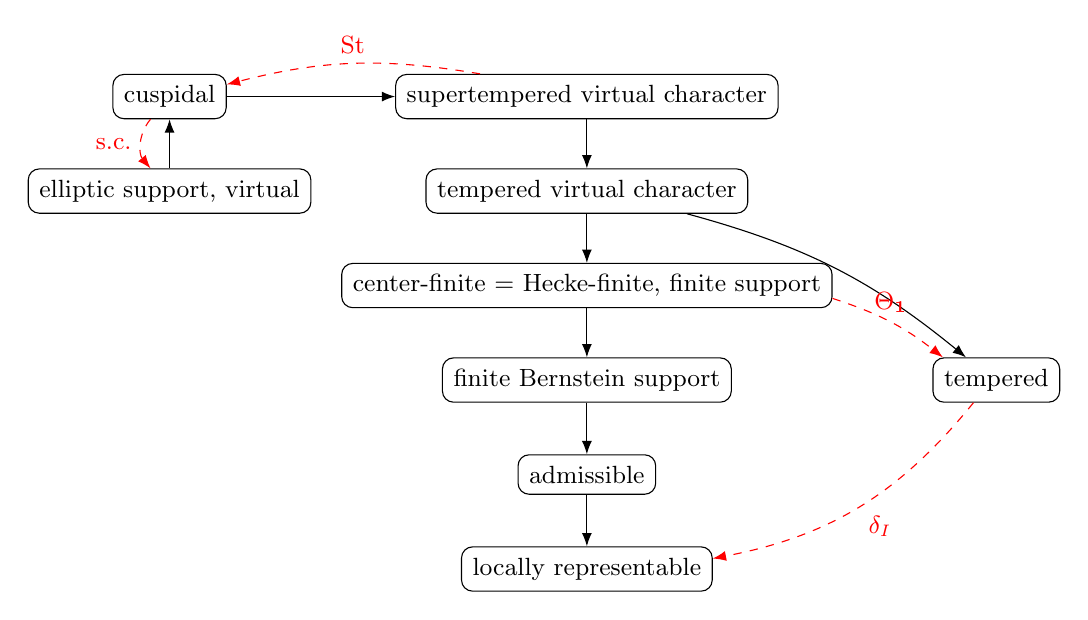
\begin{tikzpicture}[>=Latex,every node/.style={font=\small},bx/.style={draw,rounded corners,inner sep=4pt}]
\node[bx] (st) at (0,3.6) {supertempered virtual character};
\node[bx] (vc) at (0,2.4) {tempered virtual character};
\node[bx] (cf) at (0,1.2) {center-finite $=$ Hecke-finite, finite support};
\node[bx] (fb) at (0,0) {finite Bernstein support};
\node[bx] (ad) at (0,-1.2) {admissible};
\node[bx] (re) at (0,-2.4) {locally representable};
\node[bx] (cu) at (-5.3,3.6) {cuspidal};
\node[bx] (el) at (-5.3,2.4) {elliptic support, virtual};
\node[bx] (te) at (5.2,0) {tempered};
\draw[->] (st)--(vc);\draw[->] (vc)--(cf);\draw[->] (cf)--(fb);\draw[->] (fb)--(ad);\draw[->] (ad)--(re);
\draw[->] (cu)--(st);\draw[->] (el)--(cu);
\draw[->] (vc) to[bend left=12] (te);
\draw[->,dashed,red] (te) to[bend left=20] node[below right]{$\delta_I$} (re);
\draw[->,dashed,red] (cf) to[bend left=10] node[above]{$\Theta_{\triv}$} (te);
\draw[->,dashed,red] (st) to[bend right=12] node[above]{$\St$} (cu);
\draw[->,dashed,red] (cu) to[bend right=40] node[left]{s.c.} (el);
\end{tikzpicture}
\caption{Implications among the classes. Solid arrows are theorems above or in Section 8 of Draft 3. Dashed red arrows are false, with the witness named.}\label{fig:global}
\end{figure}

\section{Mistakes and inconsistencies found in earlier sections}
\begin{enumerate}[leftmargin=*]
\item \textbf{1994 notes, Section 4.2.6.} The supercuspidal characters are stated to vanish off the elliptic set. This is false, by Proposition \ref{prop:sc} and by $c_0(\pi)=-d(\pi)/d(\St)\neq0$. Draft 3 does not repeat the claim, but the restoration inventory should record it, and nothing should be restored that relies on it.
\item \textbf{1994 notes, Section 9.1.} ``A Hecke-finite distribution is a virtual character, hence automatically admissible.'' False as stated (Proposition \ref{prop:hecke}). The definition of supertempered there does not say which constant term $D_P$ is meant. With the ordinary one, Steinberg is not supertempered, which contradicts the next sentence of the notes.
\item \textbf{Draft 3, Theorem 9.1.} ``Spanned by the virtual characters arising from the elliptic constituents of tempered parabolic induction.'' The constituents $\pi_\eta^\pm$ are elliptic representations and their characters are not supertempered. The statement should name Arthur's $\Theta(M,\sigma,r)$ with $r$ regular, as in \cite[Theorem 3.1]{He94}.
\item \textbf{Draft 3, Section 9 and Glossary.} ``Retains tempered exponents'' should read ``retains the unitary exponents.''
\item \textbf{Draft 3, Theorem 8.8 and the sentence after it.} The theorem is correct for one block. The text says no criterion is asserted with supercuspidal blocks. The criterion exists (Corollary \ref{cor:descent}), and Example \ref{ex:cancel} shows that $\beta=0$ is not the right condition in general.
\item \textbf{Draft 3, Section 7.7.} ``The subspace with zero polynomial moments in the chosen unramified splitting is spanned by the quadratic character difference and the Steinberg character.'' True for the splitting $(Q,d,b)$, and it should say that the subspace changes with the splitting. Section 3.8 uses $d_{\St}=\tr\St-\tr\triv$, for which the subspace is different (Theorem \ref{thm:twosplit}). The revision log mentions the conversion. The text does not.
\item \textbf{Draft 3, Section 8.10.} ``Hecke-finiteness \dots is not a synonym for center-finiteness.'' With the 1994 definition it is, block by block (Proposition \ref{prop:hecke}).
\item \textbf{Hypotheses on $F$.} Section 1 allows any non-archimedean local field of odd residue characteristic. Section 3 assumes a finite extension of $\mathbb Q_p$. Sections 8 and 9 use Harish-Chandra's regularity theory and Herb's theorem, which are in characteristic zero. The Introduction should state the restriction once.
\item \textbf{Structure of the assembled file.} The trace comparison module begins with a subsection command, so its parts become Subsections 5.4 to 5.10 of the cocenter section, although its text says ``this section.'' The subsection ``The bilateral Laurent criterion'' follows the input of the spectral duality module and so lands at the end of Section 7, where it duplicates Theorem 7.1. The numbers ``Theorem 8.3, 8.5, 8.6, 8.8'' and ``6.1, 7.2, 7.3'' used above are my count from the source, since no combined PDF exists. They must be replaced by label references.
\end{enumerate}

\section{Inputs, verification levels and literature}
\subsection*{Classical inputs used}
\begin{center}\small
\begin{tabularx}{\linewidth}{@{}p{.33\linewidth}p{.2\linewidth}X@{}}\toprule
Input & Source & Level in this pass\\\midrule
Classification of the tempered dual; reducibility & \cite{GG63,Si79} & 3 (memory)\\
Geometric lemma, Frobenius reciprocity & \cite{Ca93} & 3\\
Character equals Jacquet character on contracting elements & \cite{Ca77} & 3, checked on four families\\
Local boundedness; local character expansion; $c_0$ and formal degree & \cite{HC99} & 3\\
Whittaker models and regular orbits & \cite{Ro75} & 3\\
Supertempered $\Leftrightarrow$ weak constant terms vanish; spanning; vanishing on elliptic set & \cite{He94}, Theorems 2.5, 3.1, 3.2 & 2. The statements were read. The displayed inequalities did not extract and were written from memory\\
Elliptic virtual characters, $R$-group inner product & \cite{Ar93} & 2 for formula $(1^*)$ of the introduction\\
$R$-groups of $\mathrm{SL}_n$ & \cite{Ke82} & 3\\
Character formula at elliptic elements & \cite{SS97}, III.4 & 2 through \cite{Ko04}. The level $e=0$ is not checked\\
Truncated formula for compact elements, rank one & \cite{Ko04} & 2 (introduction only)\\
Iwahori and principal series Hecke algebras & \cite{Bo76,Ro98} & 3\\
Trace Paley--Wiener, density & \cite{BDK86,Ka86} & 3\\\bottomrule
\end{tabularx}
\end{center}
\subsection*{Before 1994}
Harish-Chandra introduced supertempered distributions for real groups \cite{HC83}. Casselman related characters to Jacquet modules \cite{Ca77}. Kazhdan introduced the elliptic pairing and showed that restriction to the elliptic set kills exactly the induced classes \cite{Ka86}. Bernstein, Deligne and Kazhdan built the filtration of the Grothendieck group by induction \cite{BDK86}. Keys computed the $R$-groups \cite{Ke82}. Labesse and Langlands described the packets of $\mathrm{SL}_2$ \cite{LL79}. Arthur defined the elliptic tempered characters and computed their inner products \cite{Ar93}. Herb proved the three theorems quoted in Subsection \ref{sub:herb} \cite{He94}.
\subsection*{After 1994}
Schneider and Stuhler proved that the Euler--Poincar\'e pairing is the elliptic pairing and gave the fixed-point character formula \cite{SS97}. Korman extended the formula to compact elements in rank one \cite{Ko04}. Reeder related the elliptic space of Iwahori-spherical representations to elliptic representations of Weyl groups \cite{Re01}. Dat studied the cocenter and the elliptic projector \cite{Da00}. Opdam and Solleveld computed extensions of tempered representations and recovered Arthur's formula \cite{OS13}. Ciubotaru and He studied elliptic and rigid cocenters \cite{CH17,CH21}. Adler, DeBacker, Sally and Spice proved the supercuspidal character formulas \cite{ADSS11}, and Aubert and Plymen compared them with the endoscopic identities \cite{AP24}. I consulted only abstracts or introductions of the works in this paragraph, apart from \cite{Ko04}.

\section{Recommended organization of Section 9}
\begin{enumerate}[leftmargin=*]
\item[9.1] \emph{Six notions.} Definition \ref{def:six}, the example after it, and Figure \ref{fig:nested}.
\item[9.2] \emph{Constant terms.} Table \ref{tab:four}, Propositions \ref{prop:cass} and \ref{prop:bohr}. This replaces the first subsection of the 1994 Section 9 and corrects its ambiguity.
\item[9.3] \emph{Herb's theorem in rank one.} Theorem \ref{thm:herb}, Corollaries \ref{cor:irr} and \ref{cor:1994}. The two 1994 questions appear here as questions with answers.
\item[9.4] \emph{The quadratic constituents.} Theorems \ref{thm:Deta} and \ref{thm:tree}, Proposition \ref{prop:pseudo}. This restores and completes the 1994 example.
\item[9.5] \emph{The elliptic quotient.} Theorems \ref{thm:twosplit} and \ref{thm:exact}, Figure \ref{fig:splittings}. The Steinberg coordinate is treated here.
\item[9.6] \emph{Weak constant terms of distributions.} Definition \ref{def:wct}, Theorem \ref{thm:decomp}. This is the link to Section 8.
\item[9.7] \emph{Behavior at $\pm I$.} Theorem \ref{thm:germ}, Proposition \ref{prop:sc}, Corollary \ref{cor:descent}, Figure \ref{fig:cancel}.
\item[9.8] \emph{The Bernstein center and Hecke-finiteness.} Propositions \ref{prop:center} and \ref{prop:hecke}.
\item[9.9] \emph{Euler--Poincar\'e pairings.} Proposition \ref{prop:EP}, Example \ref{ex:norm}, Figure \ref{fig:grid}.
\item[9.10] \emph{Examples and counterexamples.} The table for $\mathbb Q_3$ and $\mathbb Q_5$, the list, Example \ref{ex:poisson}.
\item[9.11] \emph{Global characterization.} Theorem \ref{thm:global}, Figure \ref{fig:global}, and open problems.
\end{enumerate}
Open problems to list at the end: a description of all virtual characters with elliptic support, which needs the full supercuspidal character table on $A^0$; the admissibility of $\delta_{\rm cusp}$ (Remark \ref{rem:infinite}); explicit tree formulas for the ramified $D_\eta$ through the Type II Hecke algebra; and the metaplectic analog, where the $R$-groups and the Steinberg line both change.

Before any of this goes into the paper I recommend three audits. First, read \cite{Ca77}, \cite[Section III.4]{SS97} and \cite{HC99} for the exact statements and hypotheses used in Propositions \ref{prop:cass} and \ref{prop:sc} and Theorems \ref{thm:tree} and \ref{thm:germ}. Second, compare Proposition \ref{prop:sc} and Theorem \ref{thm:tree} with the tables of \cite{SS68,ADSS11}. Third, have Proposition \ref{prop:hecke} written out in full and refereed, since it overturns a lemma of the original notes.

\begin{thebibliography}{ADSS11}
\bibitem[ADSS11]{ADSS11} J. D. Adler, S. DeBacker, P. J. Sally, Jr., and L. Spice, \emph{Supercuspidal characters of $\mathrm{SL}_2$ over a $p$-adic field}, Contemp. Math. \textbf{543} (2011). arXiv:1012.5548.
\bibitem[AP24]{AP24} A.-M. Aubert and R. Plymen, \emph{Comparison of the Sally--Shalika character formulas with the endoscopic character identities for $\mathrm{SL}_2$}, arXiv:2410.20183.
\bibitem[Ar93]{Ar93} J. Arthur, \emph{On elliptic tempered characters}, Acta Math. \textbf{171} (1993), 73--138.
\bibitem[BDK86]{BDK86} J. Bernstein, P. Deligne, and D. Kazhdan, \emph{Trace Paley--Wiener theorem for reductive $p$-adic groups}, J. Analyse Math. \textbf{47} (1986), 180--192.
\bibitem[Bo76]{Bo76} A. Borel, \emph{Admissible representations of a semi-simple group over a local field with vectors fixed under an Iwahori subgroup}, Invent. Math. \textbf{35} (1976), 233--259.
\bibitem[Ca77]{Ca77} W. Casselman, \emph{Characters and Jacquet modules}, Math. Ann. \textbf{230} (1977), 101--105.
\bibitem[Ca93]{Ca93} W. Casselman, \emph{Introduction to the theory of admissible representations of $p$-adic reductive groups}, unpublished notes, 1974--1993.
\bibitem[CH17]{CH17} D. Ciubotaru and X. He, \emph{Cocenters and representations of affine Hecke algebras}, J. Eur. Math. Soc. \textbf{19} (2017), 3143--3177.
\bibitem[CH21]{CH21} D. Ciubotaru and X. He, \emph{Cocenters of $p$-adic groups, III: elliptic and rigid cocenters}, arXiv:1703.00378. Journal data not verified.
\bibitem[Da00]{Da00} J.-F. Dat, \emph{On the $K_0$ of a $p$-adic group}, Invent. Math. \textbf{140} (2000), 171--226.
\bibitem[GG63]{GG63} I. M. Gelfand and M. I. Graev, \emph{Representations of a group of the second order with elements from a locally compact field}, Russian Math. Surveys \textbf{18} (1963), 29--100.
\bibitem[HC83]{HC83} Harish-Chandra, \emph{Supertempered distributions on real reductive groups}, Adv. Math. Suppl. Stud. \textbf{8} (1983), 139--158.
\bibitem[HC99]{HC99} Harish-Chandra, \emph{Admissible Invariant Distributions on Reductive $p$-adic Groups}, notes by S. DeBacker and P. J. Sally, Jr., Univ. Lecture Ser. \textbf{16}, Amer. Math. Soc., 1999.
\bibitem[He94]{He94} R. A. Herb, \emph{Supertempered virtual characters}, Compositio Math. \textbf{93} (1994), 139--154.
\bibitem[Ka86]{Ka86} D. Kazhdan, \emph{Cuspidal geometry of $p$-adic groups}, J. Analyse Math. \textbf{47} (1986), 1--36.
\bibitem[Ke82]{Ke82} C. D. Keys, \emph{On the decomposition of reducible principal series representations of $p$-adic Chevalley groups}, Pacific J. Math. \textbf{101} (1982), 351--388. Pages from memory.
\bibitem[Ko88]{Ko88} R. Kottwitz, \emph{Tamagawa numbers}, Ann. of Math. \textbf{127} (1988), 629--646.
\bibitem[Ko04]{Ko04} J. Korman, \emph{A character formula for compact elements (the rank one case)}, arXiv:math/0409292.
\bibitem[LL79]{LL79} J.-P. Labesse and R. P. Langlands, \emph{$L$-indistinguishability for $\mathrm{SL}(2)$}, Canad. J. Math. \textbf{31} (1979), 726--785.
\bibitem[OS13]{OS13} E. Opdam and M. Solleveld, \emph{Extensions of tempered representations}, Geom. Funct. Anal. \textbf{23} (2013), 664--714. arXiv:1105.3802. Last page from memory.
\bibitem[Re01]{Re01} M. Reeder, \emph{Euler--Poincar\'e pairings and elliptic representations of Weyl groups and $p$-adic groups}, Compositio Math. \textbf{129} (2001), 149--181. Pages from memory.
\bibitem[Ro75]{Ro75} F. Rodier, \emph{Mod\`ele de Whittaker et caract\`eres de repr\'esentations}, Lecture Notes in Math. \textbf{466}, Springer, 1975, 151--171.
\bibitem[Ro98]{Ro98} A. Roche, \emph{Types and Hecke algebras for principal series representations of split reductive $p$-adic groups}, Ann. Sci. \'Ecole Norm. Sup. \textbf{31} (1998), 361--413.
\bibitem[Si79]{Si79} A. J. Silberger, \emph{Introduction to Harmonic Analysis on Reductive $p$-adic Groups}, Math. Notes \textbf{23}, Princeton Univ. Press, 1979.
\bibitem[SS68]{SS68} P. J. Sally, Jr. and J. A. Shalika, \emph{Characters of the discrete series of representations of $\mathrm{SL}(2)$ over a local field}, Proc. Natl. Acad. Sci. USA \textbf{61} (1968), 1231--1237.
\bibitem[SS97]{SS97} P. Schneider and U. Stuhler, \emph{Representation theory and sheaves on the Bruhat--Tits building}, Publ. Math. Inst. Hautes \'Etudes Sci. \textbf{85} (1997), 97--191.
\end{thebibliography}
\end{document}
